% !TEX root = report.tex

\section{Results}
\label{sec:results}

All numbers come from the stored notebook outputs, one run per configuration,
under the same protocol: train on $S1$, test on the unseen $S2$--$S7$.
\tab{tab:compare} collects them per measurement set and \fig{fig:perset} plots
the four milestones; \tab{tab:versions} maps each column to the change that
produced it.

\subsection{Baseline}
On the pooled unseen test set the baseline reaches $\mathbf{48.2\%}$ accuracy
(test loss $1.052$), from $45.5\%$ ($S2$) to $52.3\%$ ($S7$). Its confusion matrix
(\fig{fig:cm}\,(a)) shows two dominant error modes: \emph{sitting still} is
absorbed by \emph{empty} ($L\!\rightarrow\!E$: $0.76$), both being near-static and
concentrated at zero Doppler velocity, and \emph{running}/\emph{walking} are
heavily confused with each other ($0.39$ and $0.28$).

\subsection{Contrastive representation}
The linear probe on the frozen SupCon encoder raises overall accuracy to
$\mathbf{53.1\%}$ (validation $58.3\%$): $+4.9$ points, and an improvement on
\emph{every} set, the largest on $S3$ ($+8.3$, unseen person) and $S7$ ($+5.9$,
all conditions new). Its confusion matrix (\fig{fig:cm}\,(b)) sharpens
\emph{running} and softens the $L\!\rightarrow\!E$ confusion
($0.76\!\rightarrow\!0.52$). \emph{End-to-end fine-tuning} then \emph{hurts},
dropping back to $48.4\%$: freezing the pre-trained encoder is what generalizes,
while fine-tuning re-overfits the single training environment.

The t-SNE projection (\fig{fig:tsne}, from the sliding-window run of
\secref{sec:sliding}) is the most informative diagnostic. Colored by
\emph{environment} (right) the points are thoroughly mixed---the
SupCon objective \emph{did} reach its design goal of an environment-invariant
representation. Colored by \emph{activity} (left) the space splits into a
static region (\emph{empty}, \emph{sitting}) and a moving arc (\emph{jumping},
\emph{running}, \emph{walking}), but the activities \emph{within} each region
stay partly entangled: contrastive learning removed the \emph{domain} nuisance
and exposed a harder, intrinsic limit---a single-antenna $\approx\!2$\,s window
does not fully separate the activities, whichever way it is encoded.
Consistently, in both runs the SupCon loss fell only from $\approx\!4.6$ to
$\approx\!4.3$: the pre-training never fully converged.

\begin{figure*}[t]
  \centering
  \begin{subfigure}{0.245\textwidth}
    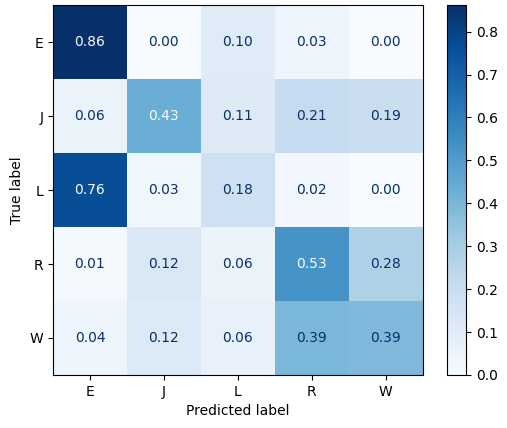
\includegraphics[width=\textwidth]{confusion_overall_c.png}
    \caption{baseline, non-overlapping}
  \end{subfigure}\hfill
  \begin{subfigure}{0.245\textwidth}
    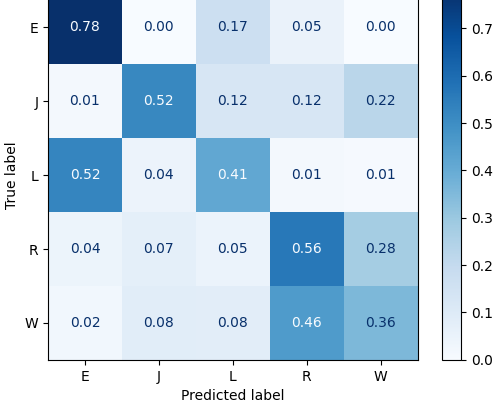
\includegraphics[width=\textwidth]{cl_confusion_c.png}
    \caption{$+$ SupCon linear probe}
  \end{subfigure}\hfill
  \begin{subfigure}{0.245\textwidth}
    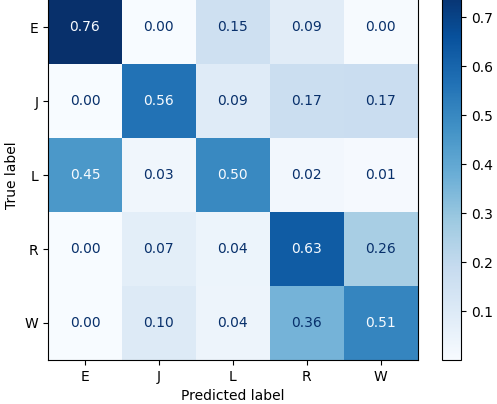
\includegraphics[width=\textwidth]{confusion_v4_single_c.png}
    \caption{baseline, sliding window}
  \end{subfigure}\hfill
  \begin{subfigure}{0.245\textwidth}
    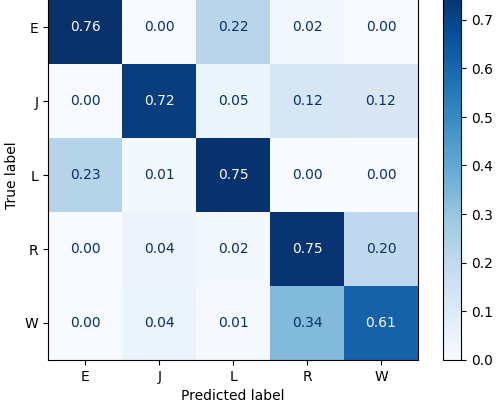
\includegraphics[width=\textwidth]{confusion_v4_fused_c.png}
    \caption{$+$ $4$-antenna fusion}
  \end{subfigure}
  \caption{Row-normalized confusion matrices on all unseen test environments,
  along the four milestones of \fig{fig:perset}. The contrastive representation
  (b) softens the $L\!\rightarrow\!E$ confusion of the baseline (a); the sliding
  window (c) lifts every class; fusion (d) then repairs the low-motion pair
  itself, $L$ going from $0.50$ to $0.75$ correct with the \emph{same} weights.}
  \label{fig:cm}
\end{figure*}

\begin{figure}[t]
  \centering
  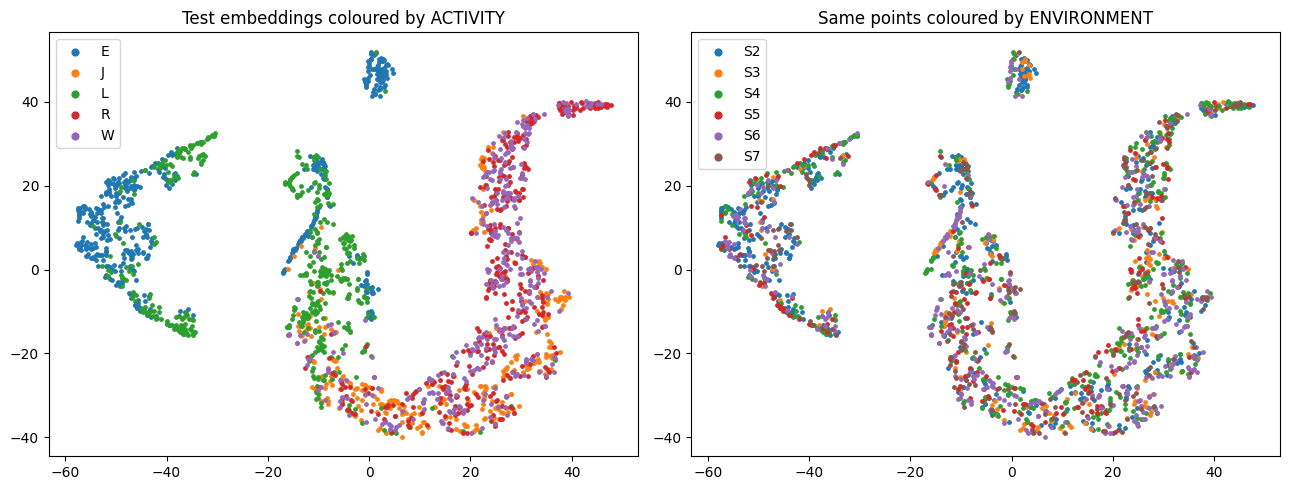
\includegraphics[width=\columnwidth]{tsne_slide.png}
  \caption{t-SNE of the test embeddings of the SupCon encoder (sliding-window
  run). \emph{Left},
  colored by activity: a static region (\emph{empty}, \emph{sitting}) and a
  moving arc (\emph{jumping}, \emph{running}, \emph{walking}). \emph{Right}, the
  same points colored by environment: the colors are mixed \emph{inside} the
  structure, i.e.\ the space is organized by \emph{activity}, not by
  \emph{environment}.}
  \label{fig:tsne}
\end{figure}

\subsection{Optimizer schedule}
The slow schedule changes only the learning rate, the patience and the epoch
budget, so the two runs isolate that factor. Slowing
training down \emph{improves} cross-domain accuracy from $48.2\%$ to $51.3\%$
($+3.1$ points, five sets out of six) even though the model fits its own training
data \emph{worse} ($0.575$ vs.\ $0.601$, \fig{fig:curves}). With a single
training environment the two objectives conflict: an epoch spent fitting $S1$
better is also an epoch spent memorizing its room, person and day. It also
tempers the previous subsection---$+3.1$ of the contrastive model's $+4.9$ points
can be bought with an optimizer setting alone, so single-run gains of a few
points here are fragile.

\subsection{Sliding-window front-end}
\label{sec:sliding}
Cutting the same recordings at stride $30$ instead of $340$ turns $13{,}564$
windows into $152{,}320$ and takes the \emph{unchanged} architecture from
$48.2\%$ to $\mathbf{59.3\%}$ ($+11.1$ points), improving every measurement set
by $8.4$ to $15.3$ points. Two caveats keep this honest: the run also raises the
early-stopping patience from $7$ to $12$, so a small part of the gain belongs to
the longer schedule; and the extra windows are strongly
correlated, so the effective sample size grows far less than tenfold. The cost is
real---$\approx\!21$\,GB of resident memory and an epoch an order of magnitude
slower, which is exactly why the loader had to allocate once instead of
concatenating---but the payoff is the single largest gain from the data side, and
it confirms that the reference implementation's stride is not an arbitrary
choice. \fig{fig:curves}(c) shows the model now reaching $0.756$ training
accuracy with validation accuracy $12$ points above the non-overlapping run, i.e.\
the denser windows buy genuine fitting capacity rather than only noise.

\subsection{Multi-antenna decision fusion}
Averaging the four per-antenna probability vectors (\eq{eq:fusion}) is the
largest single improvement we measured, and it is free: no retraining, no extra
parameters, one softmax and one group-average at inference. On the
sliding-window model it lifts $59.3\%$ to $\mathbf{72.1\%}$ ($+12.8$ points, from
$+6.9$ on $S7$ to $+17.1$ on $S2$); on the non-overlapping model it gave $+10.2$
($51.3\!\rightarrow\!61.5\%$). The gain is therefore robust to the data regime.

Its mechanism, though, changes with that regime. At stride $340$
(\tab{tab:compare}) fusion sharpened the motion classes but left
\emph{sitting}$\rightarrow$\emph{empty} untouched: with almost no motion in a
window the four antennas simply agreed on the same wrong answer. At stride $30$
the single-antenna model is already half-right on that pair
(\fig{fig:cm}\,(c), $L$ at $0.50$), and fusion converts it into the largest
per-class gain of all---$L$ reaches $0.75$ and $L\!\rightarrow\!E$ falls from
$0.45$ to $0.23$ (\fig{fig:cm}\,(d))---alongside \emph{jumping}
($0.56\!\rightarrow\!0.72$) and \emph{running} ($0.63\!\rightarrow\!0.75$).
Averaging only helps where the individual antennas disagree; denser temporal
coverage is what creates that disagreement on low-motion windows.

\begin{figure}[t]
  \centering
  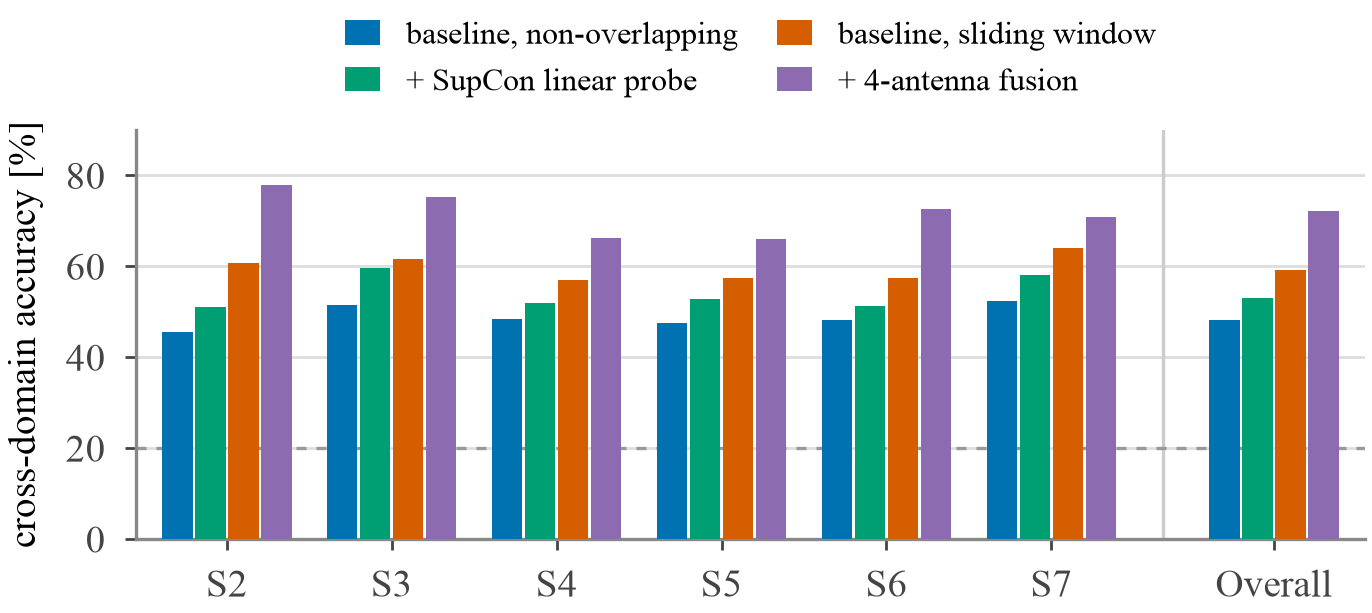
\includegraphics[width=\columnwidth]{perset_accuracy.png}
  \caption{Cross-domain accuracy per measurement set along the four milestones
  (dashed line: the $20\%$ chance level). Every unseen set benefits from the
  sliding window and, on top of it, from antenna fusion.}
  \label{fig:perset}
\end{figure}

\subsection{Does contrastive learning still help?}
Repeating the contrastive stage on the sliding-window data answers a question the
first experiment could not: the linear probe now reaches $58.3\%$, i.e.\ $1.0$
point \emph{below} the plain baseline it beat by $4.9$ points in the data-poor
regime, and fine-tuning again does worse ($57.0\%$). Read together with
\tab{tab:compare}, the contrastive stage behaves as a \emph{data-efficiency}
mechanism rather than a domain-invariance mechanism per se: when only $2767$
training windows are available it buys a representation that plain cross-entropy
cannot learn, and when $31{,}103$ (correlated) windows are available
cross-entropy catches up on its own. One confound deserves mention: the
contrastive and probe learning rates were left at $10^{-4}$ in that run while the
baseline used $10^{-3}$, so part of the one-point deficit may be an under-trained
encoder rather than the data regime.

\subsection{Comparison with the SHARP paper}
\tab{tab:compare} places our results next to the SHARP paper~\cite{sharp}: the
\emph{full} system (strongest-path sanitization $+$ 4-antenna fusion) and an
\emph{ablation} that swaps the strongest-path sanitization for the standard
reference-antenna method, feeding the \emph{same} CNN (\cite{sharp}, Table~4).
Full SHARP stays above $95\%$ everywhere. Our best configuration
(sliding window $+$ fusion, $72.1\%$) beats the ablation on \emph{every} unseen
set, by $10.6$ points ($S7$) to $26.8$ points ($S5$), and its margin is largest
exactly where the ablation collapses---the blocked-line-of-sight sets $S4$ and
$S5$. The residual $\sim\!26$-point gap to full SHARP is thus concentrated in the
one ingredient we do not implement, the strongest-path phase sanitization. The
acquisition campaigns behind the dataset also spanned nearly two years
(\cite{sharp}, Sec.~5.2), and that time diversity is itself part of what the
reference results build on.

\begin{table*}[t]
  \centering
  \caption{Per-set accuracy (\%), training on $S1$ and testing on the unseen
  sets, one run per column. Non-overlapping windows: baseline under the fast
  ($10^{-3}$) and slow ($10^{-4}$) schedules, SupCon linear probe, and fusion on
  the slow-schedule model. Sliding window (stride $30$): baseline, SupCon probe
  and fusion. Fusion always re-uses the weights of the baseline to its left.
  SHARP columns from~\cite{sharp} (Tables~3 and~4).}
  \label{tab:compare}
  \setlength{\tabcolsep}{5pt}
  \small
  \begin{tabular}{@{}lcccccccccc@{}}
    \toprule
     & \multicolumn{4}{c}{\textbf{Non-overlapping windows}}
     & \multicolumn{3}{c}{\textbf{Sliding window (stride 30)}}
     & \multicolumn{2}{c}{\textbf{SHARP~\cite{sharp}}}\\
    \cmidrule(lr){2-5}\cmidrule(lr){6-8}\cmidrule(lr){9-10}
    Set & Base (fast) & SupCon & Base (slow) & $+$ Fusion
        & Base & SupCon & $+$ Fusion & Full & Abl.\\
    \midrule
    $S2$ & $45.5$ & $51.1$ & $50.9$ & $62.6$ & $60.8$ & $59.3$ & $77.9$ & $99.8$ & $59.8$\\
    $S3$ & $51.4$ & $59.7$ & $55.9$ & $68.8$ & $61.6$ & $61.5$ & $75.2$ & $99.3$ & $58.0$\\
    $S4$ & $48.5$ & $51.9$ & $50.6$ & $58.1$ & $56.9$ & $55.6$ & $66.2$ & $97.6$ & $43.5$\\
    $S5$ & $47.5$ & $52.9$ & $49.8$ & $57.5$ & $57.4$ & $55.3$ & $66.0$ & $96.6$ & $39.2$\\
    $S6$ & $48.1$ & $51.3$ & $50.6$ & $57.9$ & $57.4$ & $56.5$ & $72.7$ & $99.8$ & $59.4$\\
    $S7$ & $52.3$ & $58.2$ & $51.5$ & $68.9$ & $64.0$ & $65.3$ & $70.9$ & $96.0$ & $60.3$\\
    \midrule
    \textbf{Overall} & $48.2$ & $53.1$ & $51.3$ & $61.5$ & $59.3$ & $58.3$ &
    $\mathbf{72.1}$ & $\sim\!98$ & $\sim\!53$\\
    \bottomrule
  \end{tabular}
\end{table*}

\subsection{Discussion}
\label{sec:discussion}

\paragraph{What each change bought}
Ranked by measured effect, decision fusion ($+12.8$) and the sliding window
($+11.1$) dominate the contrastive representation ($+4.9$, and $-1.0$ once data
is plentiful) and the optimizer schedule ($+3.1$). The ordering is a finding in
itself: the two cheapest changes---a stride constant and a few lines of
post-processing over information already present in the dataset---beat the one
that cost the most design effort, and they compose, taking the \emph{same}
$128{,}535$-parameter network from $48.2\%$ to $72.1\%$. It also matches SHARP's
own ablation, where accuracy grows monotonically with the number of fused
antennas~\cite{sharp}.

\paragraph{Why we are still far from SHARP}
The gap is now essentially one component. SHARP uses the \emph{strongest}
multipath component as phase reference, and its ablation shows the standard
reference-antenna method makes the \emph{same} CNN collapse from $>95\%$ to
$39$--$60\%$ (\tab{tab:compare}, last column). Our best model sits $10$ to $27$
points \emph{above} that ablation, so we have reproduced the decision-level half of
SHARP's robustness and improved on the data side, but none of its
signal-processing half. Training on one small environment also makes every number
high-variance.

\paragraph{Where representation learning fits}
The SupCon stage attacks domain shift on the \emph{representation} axis and, as
the t-SNE shows, succeeds there; but its measured advantage evaporates when the
front-end supplies ten times more windows. The practical reading is that
contrastive pre-training is worth its complexity when labelled windows are
scarce---which is the realistic setting for a new deployment with one calibration
environment---while in the data-rich regime the effort is better spent on the
front-end and on the decision rule. The experiment left undone is fusion on top
of the frozen probe with the contrastive stage re-tuned at $10^{-3}$: all the
components exist in the released code, but no run combines them.
